\chapter{Community assembly on isolated islands: macroecology meets
evolution}

\section{Introduction}

Current biodiversity is a product of speciation, extinction and
dispersal, contingent on the ecological interactions of organisms with
their biotic and abiotic environment. The evolutionary history leading
to the assembly of any given ecological community must in some way
shape current ecological assemblages. However, because the processes
of evolution and ecology occur on different temporal and spatial
scales, disentangling the relative influence of local ecological
mechanisms from historical evolutionary processes on patterns of
community structure remains a central challenge (Ricklefs, 2004).

The evolutionary processes of speciation and extinction are
classically viewed as constraints on regional species pools, occurring
in a manner largely removed from local ecology (Hubbell, 2001;
Cavender-Bares et al., 2009; Wiens, 2011). Conversely, ecological
mechanisms tend to be viewed as packing standing diversity into local
communities through consumption, competition, facilitation and, more
recently, neutral ecological drift (Hubbell, 2001; Tilman, 2004;
Bascompte and Jordano, 2007; Borer et al., 2014). While recent
theoretical advances have provided greater insight into ecological
drift (Hubbell, 2001; Rosindell and Phillimore, 2011), niche
partitioning (Tilman, 2004), competition, predation (Borer et al.,
2014) and species interaction networks (Williams and Martinez, 2000;
Brose et al., 2006), these insights typically do not contain realistic
evolutionary assumptions (Ricklefs, 2006) or ignore them entirely.

Insights into the genetic, biogeographic and selective mechanisms
leading to diversification have also emerged based on inference from
current patterns of species, genetic or phylogenetic diversity
(e.g. Wiens, 2011; Jetz etal., 2012). However, it is not possible to
use current static patterns to infer the temporal dynamics of either
the evolutionary mechanisms or their ecological consequences, nor can
we understand what constitutes meaningful change in a system without a
baseline for comparison. Here we show how testing idealized ecological
theories [such as the unified neutral theory (Hubbell, 2001) or the
maximum entropy theory of ecology (Harte, 2011)] on archipelagos
composed of islands formed in a discrete geological sequence can help
identify the shifting balance and feedback between fast-acting, local
‘ecological’ mechanisms, and longterm, large-scale evolutionary
processes in determining ecological community structure. Islands
having different ages of formation, along with discrete volcanoes
within islands, provide the opportunity to study diversification of
species and the assembly of communities in different
stages. Ecological theory provides an idealized ‘null’ baseline
against which to compare observed patterns.


\subsection{Hotspot oceanic archipelagos as model systems}

Hotspot oceanic islands are opportune model systems for studying the
interplay of local ecological mechanisms and the evolutionary drivers
of biodiversity patterns. Due to their sequential formation as the
tectonic plate moves over a volcanic hotspot, such island systems
offer a range of spatial and temporal scales over which to analyze the
outcomes of ecological and evolutionary processes (Warren et al.,
2015). While many archipelagos around the world share these biotic and
geological properties, the Hawaiian archipelago provides a
particularly useful system for study because its linear geological
chronology (Price and Clague, 2002), ecosystem developmental
trajectories (Vitousek, 2004) and phylogeographic patterns of
biodiversity are each well characterized (Wagner and Funk,
1995). Moreover, studies of species diversity across the islands have
revealed patterns that are non-uniform across the island
chronosequence with marked differences among lineages (e.g. Gruner,
2007; Gillespie and Baldwin, 2009) that can be used to test for
biologically meaningful differences among lineages that might drive
their disparate diversification patterns.


\subsection{Development of genetic structure}

High levels of dispersal and associated gene flow among localities
limit the extent to which populations can diverge
genetically. However, when gene flow is low, distinct populations in
different localities are free to diverge through local selective
pressures and drift, which can lead to diversification (Slatkin, 1987)
Thus, the magnitude of genetic connectivity among populations provides
a measure of the relative importance of dispersal-driven assembly
(dictated by processes removed from the local setting) in contrast to
assembly by local (in situ) diversification in determining community
composition. Using the chronosequence of the Hawaiian archipelago, we
can analyze populations from multiple sets of taxa across trophic
guilds occurring in geological contexts from young to old. We predict
that dispersal-driven (ecological) processes will dominate in
community assembly in young habitats, with the importance of in situ
(evolutionary) processes increasing with habitat age. If evolutionary
processes are not important, we predict that communities should reach
a statistical steady state through ecological processes alone (Harte,
2011). If, as we expect, evolutionary processes become increasingly
important in community assembly over time, we would expect to find
associated deviations from an ecological null model of community
assembly, provided by idealized ecological theory. Differences in
population structure among taxa or trophic groups could indicate
whether sufficient time has passed along the chronosequence for the
group of interest to experience significant evolutionary pressures.


\subsection{Macroecological metrics and idealized ecological theory}

By their nature, unified theories of biodiversity (e.g. Hubbell, 2001;
Harte, 2011) provide a simplified view of ecology, but deviations from
theory can provide insights into which particular ecological patterns
require additional biological mechanisms for their explanation (Harte,
2011). The maximum entropy theory of ecology (METE; Harte, 2011) in
particular provides predictions of species abundance distributions,
species–area relationships and metabolic rate and network linkage
distributions for idealized ecological communities in which the
behavior of a system is governed by a simple set of state
variables. The principle of maximum information entropy (MaxEnt), from
which the METE is derived, is an established inference procedure that
has yielded accurate predictions of diverse patterns in fields as
varied as thermodynamics (Jaynes, 1957), economics (Golan et al.,
1996), forensics (Roussev, 2010), imaging technologies (Gull and
Newton, 1986) and, more recently, ecology (e.g. Phillips et al., 2006;
Dewar and Porte, 2008; Harte, 2011). MaxEnt works by seeking the
least-biased prediction of a distribution of interest (e.g. the
distribution molecular velocities in the case of thermodynamics or of
species abundances in the case of ecology) while constraining that
prediction to be consistent with state variables describing the
macroscopic attributes of the system (e.g. temperature or the total
number of species and individuals). These are the most ignorant
possible predictions about the system. Thus, studying the unique
ecological conditions and evolutionary histories of real-world systems
that deviate from the conditions predicted from maximizing information
entropy can provide insights into the processes driving ecological
systems away from the statistical steady state (Harte, 2011).

Ecological networks are complex systems forming hierarchical
structures to which the principle of MaxEnt has recently been applied
(Williams, 2010; Harte, 2011) and are a prime study focus because
networks of interacting species embody both the ecology of trophic
links and evolutionary processes such as co-evolution (Bascompte and
Jordano, 2007; Donatti et al., 2011; Nuismer et al., 2013; Thompson et
al., 2013). Thus they present an opportune starting place to study
ecological and evolutionary feedbacks. The distribution of linkages in
ecological networks can test whether plant–animal interaction networks
assemble neutrally or through deterministic processes such as
co-evolution of traits involved in foraging (Vazquez et al.,
2005). Analysis of other network metrics such as modularity (the
degree to which species interact in semi-autonomous modules) and
nestedness (the degree of asymmetry in interaction between specialists
and generalists) can further illuminate the underlying
eco-evolutionary processes driving patterns of species interactions
(Bascompte and Jordano, 2007; Donatti et al., 2011; Nuismer et al.,
2013). In nested networks, species with fewer interactions (i.e. more
specialized species) will interact with a subset of the species with
which generalists interact. In this way interaction nestedness is
mathematically equivalent to island nestedness (in which islands that
are less species rich are subsets of islands that are more species
rich). However, we only consider network nestedness here.

To gain insights into community assembly as it happens, we propose an
integrative framework that harnesses advances in both evolutionary and
ecological theory, placed in the context of age-structured
archipelagos. Mechanistically simplified ecological theories such as
the METE (Harte, 2011) can be used as powerful null models; deviations
from theoretical expectations can flag biological phenomena that
warrant further study. Here we demonstrate how community-level data
from age-structured island systems, combined with population genetic
and phylogenetic data, can test the extent to which the evolutionary
histories behind such communities drive their deviation from
theoretical expectations. We provide an initial test of this concept
using a synthesis of published data on arthropod lineages in the
Hawaiian islands. We provide metrics of ecological and evolutionary
dynamics across communities from settings that range in geological age
from 500 years to 5 Ma. We estimate taxon-specific timelines for the
development of population genetic structure for both herbivores and
predators and couple these results with macroecological measures of
community structure, using predictions from statistical steady-state
and ecological network theory to provide insights into changes in
community structure over the extended timeframe provided by the island
chronosequence.


\section{Methods}

\subsection{Dispersal-driven processes to in situ differentiation
across the island chronosequence}

To evaluate the balance between regional immigration and the potential
for local differentiation, we measured how molecular variation is
partitioned among populations within species across locations of known
substrate age on the islands of Hawaii and Maui (Fig. 1). We compiled
published [DNA sequences, amplified fragment length polymorphism
(AFLPs) and allozymes] and new data sets for a diversity of native
Hawaiian arthropod groups that represent a spectrum of trophic levels
(Table1). New sequences were included for sap-feeding Hemiptera group
Nesosydne planthoppers [COI; data generated following the protocols in
Goodman et al. (2012); GenBank accession numbers: KT023113–KT023179]
and Trioza psyllids [COI, cytB; data generated following protocols in
Percy (2003); GenBank accession numbers: KR108061–KR108144]. Samples
were from the focal sites described below for the ecological analysis,
as well as from other locations across Hawaii and Maui. These data
were used to provide an estimate of how arthropod populations have
accumulated genetic population structure within the focal sites of
different geological age.

We used analysis of molecular variance (AMOVA) to examine how genetic
variation is partitioned at two scales of population structure: among
sites within volcanoes and among volcanoes on both the island of
Hawaii and the islands of the Maui Nui complex (Maui, Molokai,
Lanai). All analyses of allozyme and DNA sequence data were performed
in \texttt{Arlequin} v.3.5 (Excoffier and Lischer, 2010) using the AMOVA
procedure to compute $F_{ST}$, a measure of genetic variance, or,
where possible, $\Phi_{ST}$, an $F_{ST}$ analogue that incorporates
genetic sequence information. The Laupala AFLP data were analyzed
using \texttt{tfpga} v.1.3 (Miller, 1997), using the same hierarchical
approach of comparing within and among volcanoes as described
above. To provide a temporal framework for the population
differentiation analysis we assembled divergence-dating information
from the literature for as many of the taxa as possible.

To explicitly test the association between landscape age and the
potential for in situ genetic divergence we analyzed how within-site
$F_{ST}$ varies with the geological age of volcanoes on the islands of
Hawaii and Maui Nui. For each volcano we calculated $F_{ST}$ or
$\Phi_{ST}$ (Excoffier and Lischer, 2010) for each taxon among sites
within volcanoes. This analysis assumes that volcano age parallels
habitat age, allowing more or less time for the presence of the
populations.


\subsection{Ecological metrics across the island chronosequence}

To investigate how ecological patterns change as communities age, we
selected four focal sites across the chronosequence and island ages
(two on the island of Hawaii, one on Maui and one on Kauai; Fig. 1) of
approximately 12 km$^2$ (each was defined as a point with a 2 km radius
buffer). Focal sites were selected to have similar forest composition
(dominated by Metrosideros polymorpha; Myrtaceae), elevation
(1100–1400 m) and rainfall (mean annual precipitation 2000–3000
mm). We then constructed bipartite interaction networks between native
herbivorous Hemiptera species and native plants at each of the study
sites. Bipartite networks describe the topology of ecological
interactions between two guilds of organisms (e.g. herbivores and
their plant hosts). Quantitative information on the relative
importance of interaction links can be incorporated into network
analyses (Vazquez et al., 2009). However, currently available data are
restricted to binary networks: those that describe the potential for
interaction between any two species but not the relative frequency of
that interaction to each species.

We compiled species lists of all native herbivorous Hemiptera for each
focal site from published species accounts (see Table S1 in the
Supporting Information for a full list). Species accounts and other
published sources were used to determine the presence, probable
presence, or probable absence of each species at each of our four
focal sites. A documented presence was defined as a known specimen
collected at the focal site; a probable presence was defined as a
species whose abiotic tolerances and known geographic range overlap
with a focal site but no known specimen exists confirming its
presence. Probable absence was assumed when the criteria for presence
or for probable presence are not met. Two sets of species lists for
each focal site were compiled: a conservative data set composed of
only documented presence occurrences and a less conservative data set
that also included probable presences.

Host plants for each species of Hemiptera were determined from
published species accounts. Data on host plant use at each specific
site were not available so we assumed that if a known host plant were
present at a site it would eventually be used. Host plant occurrence
in the focal sites was determined using distribution models for 1158
species of Hawaiian plants (Price et al., 2012). Each focal site was
spatially joined in a geographic information system with all
coincident plant distribution models that fell within its
boundaries. Two sets of resulting focal site-specific networks were
constructed: one using the conservative data set of Hemiptera species
presences and the other using the less conservative data set.

We hypothesized that potentially complex evolutionary feedbacks
contributing to community assembly should result in departures from
the predicted ecological statistical steady state. We used the METE
(Williams, 2010; Harte, 2011) to compute the statistical steady state
for the distribution of the number of host plants used by each
Hemiptera species (hereafter referred to as degree distribution). To
evaluate how well the METE predicts the data we simulated
METE-conforming communities having the same number of species and
links as observed. We then calculated the log-likelihood of each
simulated data set and compared the resultant distribution of
log-likelihoods under the hypothesis that the METE is true with the
observed loglikelihood. This comparison is identical in approach to a
z-score test using a Monte Carlo simulation to estimate the sampling
distribution of log-likelihoods. \texttt{R} scripts (v.3.1.1; R Core Team,
2014) used for METE estimation and Monte Carlo methods are available
in Appendix 1.  To investigate how speciation may in part drive
network patterns and deviations from those predicted by idealized
ecological theory, we analyzed the number of links assigned to each
Hemiptera species (the degree distribution) separately for
single-island endemics (those species found on only one island and
thus probably derived from in situ diversification) versus
multi-island endemics (those species found on multiple
islands). Although multiple processes can lead to a species being a
single-island endemic (Whittaker et al., 2008), such taxa provide a
proxy for how much speciation occurs within islands. To compare
species degree distributions between single-island endemics and
multi-island endemics across sites of different ages we conducted a
generalized linear model with binomial error, treating site identity
as a categorical predictor. Binomial errors effectively account for
network size due to the bounded support of the binomial distribution.

To understand how other network properties change with age of the
ecosystem substrate, we calculated two widely used descriptive network
metrics across sites–--nestedness and modularity. Nestedness describes
the degree of asymmetry of species interactions connecting specialists
and generalists (Bascompte and Jordano, 2007; Ulrich et al., 2009). We
calculated nestedness using the NODF metric (Almeida-Neto et al.,
2008) as implemented in the R package vegan (Oksanen et al., 2013) and
modularity using a variety of algorithms implemented in the \texttt{R}
package \texttt{igraph} (Csardi and Nepusz, 2006). These metrics are not
directly comparable across networks of different size and connectance
(Ulrich et al., 2009), so for each metric in each network we calculate
z-scores using a null model that randomizes network structure while
maintaining certain aggregate network properties (Ulrich et al.,
2009). These z-scores are calculated as the difference between the
observed network metric minus the mean of the null model divided by
the null model standard deviation, or
$(x_{obs} − \bar{x}_{sim}) / SD_{sim}$. Because z-scores can be highly
sensitive to the choice of null model (Ulrich et al., 2009) we
implemented both a probabilistic null model (Bascompte and Jordano,
2007) and a null model that strictly constrains the degree
distributions of plants and herbivores (Ulrich et al., 2009). The
probabilistic null uses the frequency of interactions as the
probability that a randomized link gets assigned to that cell in the
interaction matrix (Bascompte and Jordano, 2007); thus the
probabilistic null constrains row and column sums in probability but
not absolutely.


\section{Results}

\subsection{Dispersal-driven processes to in situ differentiation
across the island chronosequence}

The AMOVA revealed significant genetic population structure from the
smallest to the largest spatial scales examined, all within a very
recent timeframe. For mitochondrial loci, statistically significant
molecular variation partitioned among sites within volcanoes ranged
from 0.037 to 0.92 and among volcanoes from 0 to 0.30. Corresponding
variation at multilocus nuclear loci among sites within volcanoes
ranged from 0.21 to 0.58 and among volcanoes from 0.04 to 0.34. Taxa
in the lower trophic levels (herbivorous sap-feeding Hemiptera:
planthoppers and psyllids) had as much or more molecular variation
partitioned at the among-site, within-volcano level than the
among-volcano level, while the predatory spiders were less structured
at localities within volcanoes compared with among them (Table 1). The
analysis of genetic population structure across the chronosequence of
localities revealed a similar pattern. The herbivores show high
genetic population structure among localities even on young volcanoes
(Fig. 2). By contrast, predatory spiders exhibited little genetic
population structure within sites on the same volcano; this was higher
among volcanoes, with values increasing with age across the
chronosequence.

The observed levels of genetic divergence have evolved rapidly in many
cases. For example, for species from the island of Hawaii for which
phylogenetic data provide divergence times, estimates of dates of
species divergence range from 0.5–4 Ma, with additional within-species
genetic divergence having developed subsequently (Table 1). That some
of these estimates are older than the known age of the ‘Big Island’
suggests that genetic divergence pre-dates their colonization to
Hawaii, or alternatively that estimates include sampling error. For
the one species where population genetic data were used to estimate
divergence times between populations, herbivorous Nesosydne
planthoppers, it was determined that populations diverged as little as
2600 years ago (Goodman et al., 2012) (Table 1).


\subsection{Ecological metrics across the island chronosequence}

The degree distribution of Hemiptera species varied across the
chronosequence with both the youngest and oldest sites deviating most
from the statistical steady-state maximum entropy predictions
(Fig. 3). In the intermediate-aged site of Kohala, deviations are not
significantly different from the predictions of maximum entropy.  The
generalized linear model revealed significant differences between the
degree distributions of single-island endemics (species whose
distributions are restricted to only one island) versus archipelagic
endemics that are found across multiple islands
(Fig. 3). Single-island endemics show significantly lower degree
distributions overall (i.e. more specialization) compared with more
generalist species found across multiple islands. Furthermore,
single-island endemics use more host plant species on the
intermediate-aged Maui site. The slightly younger Kohala shows
increased generalization for both single-island endemics and
archipelago endemics. However, when considering the degree
distribution defined by trophic links to plant genera instead of plant
species, the pattern of increased generalization holds for Kohala, but
endemics on Maui no longer show a difference in their degree
distributions from other island endemics. This change in pattern
suggests that increased generality of Maui endemics may be driven by
increased plant species diversity within genera on that island.

Network nestedness decreased with habitat age while modularity
increased (Fig. 4). This trend was recovered in networks constructed
from both more and less stringent geographic criteria
(Fig. S3). Choice of null model changed the magnitude of modularity
and the sign of nestedness z-scores; however, the relative pattern of
decreasing nestedness and increasing modularity remained across the
different null models used to standardize network metrics
(Fig. S2). The patterns were also robust to sampling intensity, as
demonstrated by a rarefaction analysis (Fig. S4).


\section{Discussion}

\subsection{Development of genetic population structure at different
trophic levels}

The analysis of available genetic data presented here indicates that
divergence is occurring within the islands at small spatial scales and
over short time periods (Table 1, Fig. 2). Furthermore, the scale of
population structure varies with trophic position, with structure
developing in sap-feeding herbivore lineages at smaller scales (and
hence shorter timeframes in the context of the chronosequence)
compared with detritivorous crickets and predatory spiders (Table 1,
Fig. 2). Structure within species may allow populations to take
independent evolutionary trajectories, especially when aided by other
evolutionary processes acting differentially across species geographic
ranges. A variety of factors have been associated with the genetic
divergence of populations and species in the lineages described here,
including combinations of genetic drift associated with geographic
isolation (Percy, 2003; Mendelson and Shaw, 2005; O’Grady et al.,
2011; Goodman et al., 2012), adaptation associated with competition,
predation and mutualism (Gillespie, 2004; Roderick and Percy, 2008;
Brewer etal., 2015) and sexual signaling (Mendelson and Shaw, 2005;
Percy et al., 2006; Magnacca et al., 2008; Goodman et al., 2015).

The Nesosydne planthoppers provide evidence that some period of
geographic isolation preceded the divergence of sexual signals
(Goodman et al., 2012, 2015). Shifts in plant host use are also
associated with diversification in this group (Roderick and Percy,
2008). In a phylogenetic study of a radiation of sap-feeding
Nesophrosyne (Cicadellidae) leafhoppers, species divergence was
associated with host plant specialization between 1 and 5 Ma, but only
with geography on the younger island (Bennett and O’Grady, 2013). Our
network analysis shows that specialization and modularity are more
pronounced on Maui than on Hawaii (Figs 3 and 4), consistent with the
phylogenetic results from Nesophrosyne. Available dating analyses of
other arthropod taxa indicate that population genetic structure can
develop in much less than 1 Myr (Table 1), and suggest that landscape
fragmentation processes (e.g. lava flows) may dominate the earliest
stages of diversification across taxa in the Hawaiian islands. Other
taxa at low trophic levels, such as the herbivorous Trioza psyllids,
detritivorous Laupala crickets and fungivorous Drosophila, show
similar signals of geographic isolation combined with ecological and
sexual processes driving genetic divergence and diversification across
sites as young as those on Hawaii (Percy, 2003; Mendelson and Shaw,
2005; Percy et al., 2006; Magnacca et al., 2008; O’Grady et al.,
2011). By contrast, spiders, which are predatory, develop genetic
discontinuities at larger spatial and temporal scales with a strong
signature of increasing structure with age of the chronosequence
(Roderick et al., 2012; Table 1). Further work is needed to assess the
generality of this pattern of slower genetic differentiation in
predators compared with herbivores.


\subsection{Macroecological metrics: network structure and steady
state}

Across the Hawaiian archipelago, nestedness appears to decrease
generally with site age, and is highest on the geologically youngest
volcano, Kilauea. High nestedness on Kilauea may arise with high
immigration of new species with high probabilities to eat or be eaten
by the generalist species already present at the site (Bascompte and
Jordano, 2007). However, despite high nestedness on Kilauea, and thus
the potential for neutral colonization-driven assembly, this site did
not conform to the statistical steady-state predication of the
METE. The observed deviations from the METE at Kilauea appear to be
largely driven by a surplus of singleton links (Fig. 3), which may
reflect a state of ‘incomplete’ assembly, possibly by lower species
richness of the plant and herbivore biotas. Conversely, at Kohala, at
intermediate age (150 ka), observations were not significantly
different from the METE predictions. We posit that the reason why
theoretical predictions fit Kohala so well is that the site has had
sufficient time to undergo ecological succession and thus arrive at a
statistical steady state, but is still too young to be affected by
ecological specialization and rapid in situ diversification associated
with host plants on older islands.

Interestingly, the communities on the older Maui and Kauai sites show
strong deviations from the METE expectations (Fig. 4). The METE is
agnostic about which mechanisms determine the values of the state
variables that lead to its macroecological predictions (Harte,
2011). It does not account for the evolutionary history of biological
systems. Thus, one possible explanation for the strong deviations from
the METE expectations, compared with observations at our
intermediate-aged site (Kohala), is that while the ages of Maui and
Kauai are sufficient for evolutionary assembly driven by
specialization and diversification on host plants, the older age of
these islands may have led to range contractions and possibly
extinction of plant species on the oldest island of Kauai (Whittaker
et al., 2008).

Our results show decreased nestedness and increased modularity on Maui
and Kauai. Co-evolution between interacting species should lead to
greater modularity (Donatti et al., 2011; Nuismer et al.,
2013). However, the influence of certain network properties, such as
nestedness, on stability is still unknown, and so theoretical
predictions of how network properties should change over evolutionary
time, generally, are lacking. Theoretical and empirical studies have
suggested that nestedness may or may not promote stability (Allesina
and Tang, 2012; Suweis et al., 2014). Furthermore, almost all studies
of food webs have focused primarily on single or short ecological time
spans of network development that do not span as much evolutionary
time as is included here (e.g. Albrecht et al., 2010). Food webs are
dynamic emergent entities, with broad topological characteristics that
may change dramatically over time (e.g. Yeakel et al., 2013). To our
knowledge, our study represents the first to evaluate network topology
over larger temporal scales, and we argue that age-structured
landscapes such as the Hawaiian archipelago are promising for
resolving long-standing debates on the causes and consequences of
network properties such as nestedness.

We found that single-island endemics were always more specialized than
multiple-island endemics. Although dietary breadth has been positively
associated with geographic range size (Lewinsohn et al., 2005), the
direction of causality is unclear (Slatyer et al., 2013): while
dietary breadth may allow some species to colonize other islands, it
may also be driven by adaptation to exploit locally abundant hosts
across a large range. Nevertheless, both scenarios are consistent with
the hypothesis that in situ formation of single-island endemics may be
the product of co-evolution and specialization. At the Kohala site,
which showed the best fit to maximum entropy theory, single-island
endemic and multiple-island endemic species alike showed increased
generalization (i.e. a higher degree, or more links; Fig 3), while at
the youngest site of Kilauea, specialist single-island endemics may be
limited by low plant diversity and thus appear more specialized
(Fig. 3). Conversely at the oldest site on Kauai, where plant
diversity is high (Kitayama and Mueller-Dombois, 1995), single-island
endemics are again associated with decreased degree and thus genuine
specialization (Fig. 3). On Maui, single-island endemics show
statistically significant increases in generalization, but this
pattern disappears when analyzing the data at the resolution of plant
genera, thus suggesting that Hemiptera species endemic to Maui may
benefit from the diversification of plant species within genera.


\subsection{Future research}

The data and analyses presented here describing insect and plant
communities across a chronosequence of habitats in Hawaii generate
testable hypotheses concerning the relative importance of ecological
and evolutionary processes in community assembly. Our work to date
suggests the overarching hypothesis that ecological processes dominate
community assembly in younger environments, with evolutionary
processes becoming increasingly important as communities age. We can
also make predictions about the sequence of community assembly based
on proposed mechanisms.

In younger communities we predict characteristics of ecological
assembly, with species resembling random samples through immigration
from regional source pools. Thus, metrics describing these communities
will approach expectations of an ecological statistical steady
state. An exception will be communities that are still undergoing the
initial stages of primary succession, which will change rapidly
through time and represent nonrandom samples of source pools. We also
predict that these communities will exhibit a nested network
structure, assuming new species will eat or be eaten by the generalist
species already present in the community, as suggested by previous
work on nestedness (Bascompte and Jordano, 2007) and by our finding
that widespread species tend to be generalists (Fig. 4).  Following
the same logic, in older communities we expect to see characteristics
of evolutionary assembly, dominated by processes such as adaptive
exploration of niche space, giving way to speciation. Thus, we predict
increasing specialization and modularity with time (Bascompte and
Jordano, 2007; Donatti et al., 2011; Nuismer et al., 2013) as
reflected by age across the chronosequence.


\subsubsection{Ecological data: assembly of species into communities}

In order to build a more rigorous understanding of the assembly
process in both younger and older communities, fine-grained sampling
of all macroscopic arthropod taxa is needed from a large number of
sites across the island chronosequence. This will allow an assessment
of changes in overall species composition and diversity across all
players in the time-calibrated landscape (Gruner, 2007). Such data
will allow us to test entire arthropod communities for deviations from
METE predictions of statistical steady state (Harte, 2011) across
substrates of different ages. For example, predators, whose
assemblages are likely to be more dominated by immigration and
ecological assembly (Fig. 2), may never show strong deviations from
METE predictions, whereas herbivores could show increasing deviation
with age in agreement with the network results of this paper (Fig. 3).


\subsubsection{Evolutionary data: diversification within species} The
current study demonstrates that taxa from different trophic guilds
differ in the scale at which differentiation occurs and highlights the
importance of fragmentation of the landscape in facilitating
differentiation. Future work will be aimed at gathering data for
additional focal taxa within this system, spanning different trophic
levels. We will use these data to understand taxonomic and functional
differences in the rate of differentiation, to assess the roles of
genetic fusion and fission and the spatial scale over which they are
important in fostering diversification (Gillespie and Roderick, 2014),
and to detail the relative rates of speciation and extinction across
the island chronosequence.


\section{Conclusions}

We have shown how a chronosequence can be used to understand
biodiversity dynamics across an ecological–evolutionary
continuum. Focusing on entire communities of arthropods in the
Hawaiian islands allows us to incorporate predictions from idealized
ecological theories to understand eco-evolutionary feedbacks and
generate predictions about how entire communities develop over an
extended time. Such an approach may prove fruitful for investigating
the separate and interactive roles of ecological and evolutionary
drivers of community assembly using age-structured systems as a
simplified natural experiment, as exemplified by oceanic archipelagos.

We have demonstrated how taxa in the lower trophic levels developed
genetic structure even in the youngest habitats of the observed
chronosequence and at smaller spatial scales (Table 1, Fig. 2). Thus,
lower trophic levels are affected by in situ processes of
diversification very early in the chronosequence, compared with higher
trophic levels, though in situ processes become more important over
time in the latter. Network nestedness decreased while modularity
increased with age (Fig. 4), again indicating a possible shift from
assembly driven by ex situ immigration early on to one based on in
situ diversification, such as in co-diversification of insect
herbivores with host plants (Bascompte and Jordano, 2007; Donatti et
al., 2011). That single-island endemics (probably the product of in
situ diversification) show more specialization at older sites than
more broadly distributed species (those taxa more likely to be initial
colonists; Fig. 3) also supports this hypothesis.

This study provides a framework for using chronologically arranged
oceanic island systems to examine the interplay between evolutionary
and ecological processes in shaping biodiversity. Our initial results
provide a clear hypothesis that ecological processes dominate
community assembly in younger environments, with evolutionary
processes becoming more important as communities age. We demonstrate
how this approach can provide insights into the development of
communities over ecological–evolutionary time, and the dynamic
feedbacks involved in assembly.


\section*{Acknowledgements} 

We are indebted to many scientists and land managers in Hawaii who
have provided access to the lands: Pat Bily (The Nature Conservancy of
Hawaii), Melissa Dean, Christian Giardina, and Tabetha Block (Hawaii
Experimental Tropical Forests), Betsy Gagne (Natural Area Reserve
System), Lisa Hadway and Joey Mello (Department of Forestry and
Wildlife Hilo), Cynthia King and Charmian Dang (Department of Land and
Natural Resources) and Rhonda Loh (Hawaii Volcanoes National Park). We
thank Robert Ricklefs, Lauren Ponisio and two anonymous referees for
thoughtful commentary. We are very grateful to Guida Santos, Richard
Field and Robert Ricklefs for inviting us to contribute to this
Special Issue. The research was supported by the National Science
Foundation DEB 1241253.


\bibliographystyle{thesis}
\bibliography{thesis}

\clearpage

\section*{Figures}

\begin{figure}
%\centerline{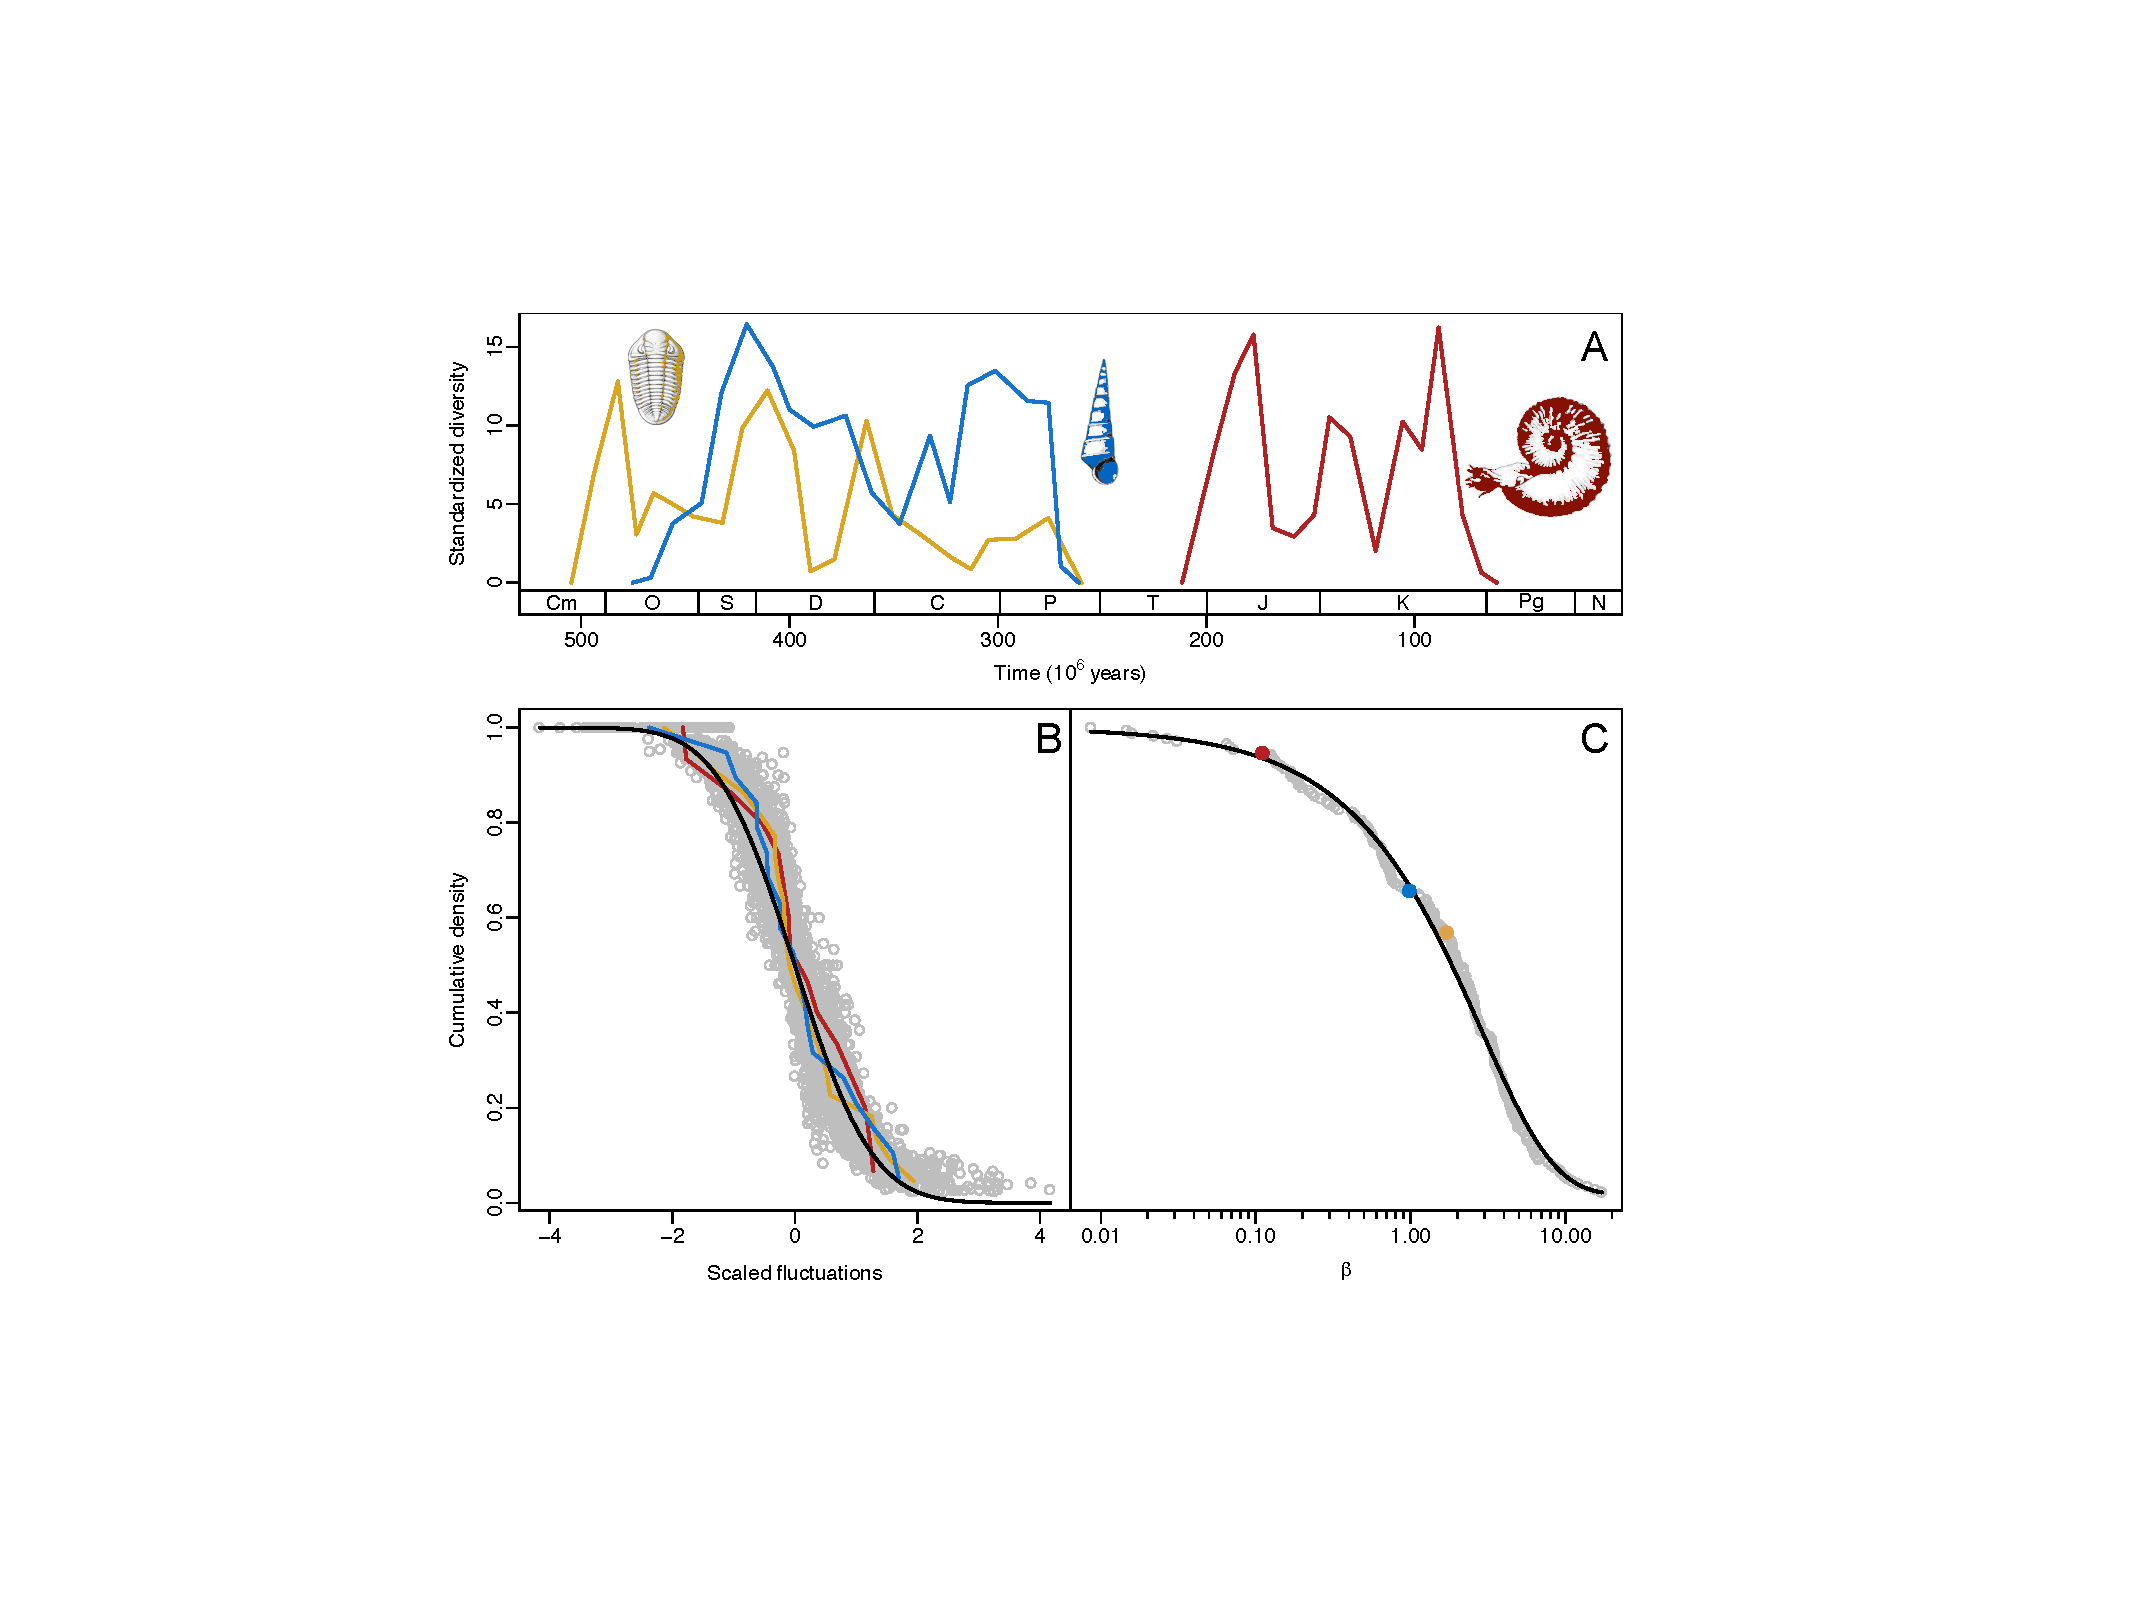
\includegraphics[scale=0.5]{fig_pkx-fbeta.pdf}}
  \caption[Map of substrate age]{Map of substrate age (millions of
    years, My) of the islands of Kauai, Maui and Hawaii. Colours
    correspond to substrate age from young (light) to old
    (dark). Focal sites are shown as black circles (on Hawaii, Kohala
    is in the north, Kilauea in the south) while sampling sites for
    genetic data are represented by grey circles..}
  \label{fig:map}
\end{figure}

\begin{figure}[!hp]
  \centering
%  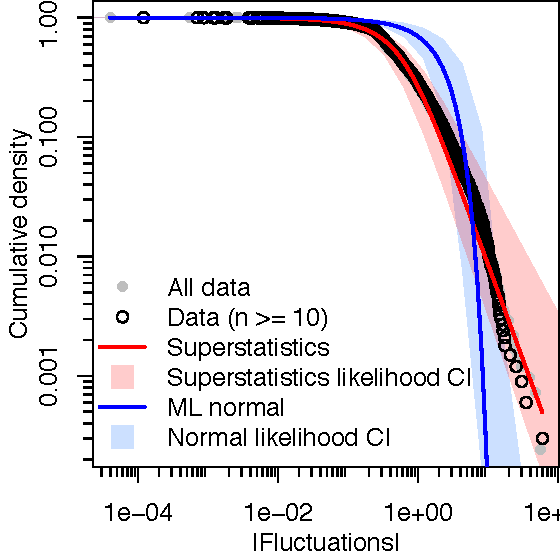
\includegraphics[scale=0.7]{fig_Px.pdf} 
  \caption[Population genetic structure]{Population genetic structure
    ($\Phi_{ST}$ for all taxa except \textit{Laupala} for which we
    used $F_{ST}$) among sites within volcanoes with volcano age for
    insects and spiders. Calculations were based on mitochondrial DNA
    only (see Table 1 for details). The plant-feeding groups,
    specifically the sap-feeding Hemiptera, show higher genetic
    structure among sites on young volcanoes relative to older
    volcanoes, whereas detritivores (crickets), fungivores
    (\textit{Drosophila}) and in particular predators (spiders) show
    little structure on young volcanoes. For spiders, substantial
    structure develops only later in the chronosequence, for example
    on Maui at approximately 1 Ma. Numbers refer to different species:
    1, \textit{Nesosydne chambersi}; 2, \textit{Nesosydne
      raillardiae}; 3, \textit{Nesosydne bridwelli}; 4,
    \textit{Trioza} HB; 5, \textit{Trioza} HC; 6, \textit{Drosophila
      sproati}; 7, \textit{Laupala cerasina}; 8, \textit{Tetragnatha
      anuenue}; 9, \textit{Tetragnatha brevignatha}; 10,
    \textit{Tetragnatha quasimodo}; 11, \textit{Theridion grallator}.}
  \label{fig:popGen}
\end{figure}

\begin{figure}[!hp]
  \centering
%  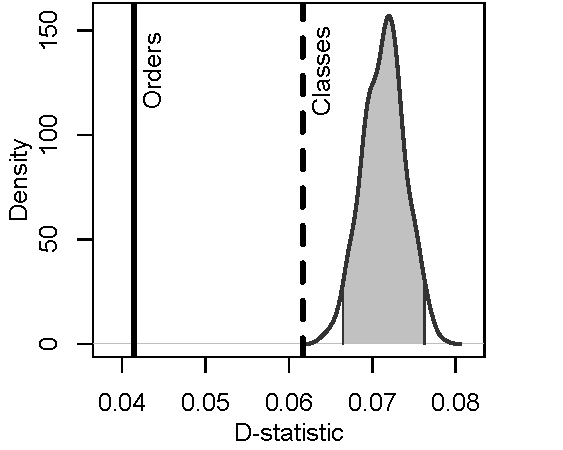
\includegraphics[scale=0.9]{fig_dStat(3TP).pdf}
  \caption[Patterns in degree distributions across sites]{Patterns in
    degree distributions across sites, comparing archipelago-wide
    endemics (cosmopolitans) with single-island endemic (Endemics)
    taxa. The top panels show that networks deviate most from the
    predictions of the maximum entropy theory of ecology on the
    youngest and oldest sites. Inset figures show the distribution of
    simulated mean squared errors; if the vertical/red line falls
    within the grey region (95\% confidence interval) the data are not
    significantly different from the predictions of maximum entropy
    theory. All sites except Kohala deviate from the predications. The
    bottom panel shows the number of links for endemics versus
    cosmopolitans. Endemics show lower linkage overall, but
    significantly increase on the intermediate-aged site Maui
    (highlighted with dotted box). Kohala shows increased linkage
    overall (highlighted with a solid box).}
  \label{fig:degree}
\end{figure}

\clearpage

\section*{Tables}

\begin{table}[!hp]
  \centering
%  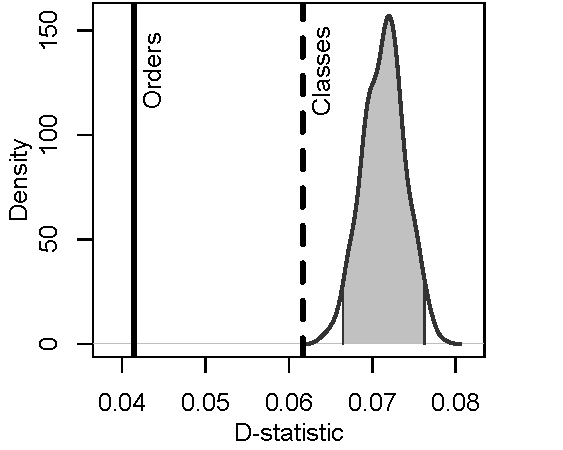
\includegraphics[scale=0.9]{fig_dStat(3TP).pdf}
  \caption[Results of the analyses of molecular variance]{Results of
    the analyses of molecular variance (AMOVA) that partitions
    molecular genetic variation among volcanoes and among sites within
    volcanoes for arthropod lineages found within the study sites on
    the island of Hawaii. Where estimates of divergence through
    molecular dating are available for the taxa, they are presented to
    show the timeframe within which this genetic structure has
    developed.}
  \label{tab:genStat}
\end{table}
